\newcommand{\comment}[1]{}


\title{\Large \bf M.Eng. Project Report Spring 2013}
\author{
{\rm OpenComm Team}
}
\date{\today}

\documentclass[12pt, letterpaper]{article}
\usepackage{fullpage}
\usepackage{graphicx}
\usepackage{epsfig}
\usepackage{algpseudocode}
\usepackage{url}
\usepackage[toc,page]{appendix}
%\usepackage[margin=0.90in]{geometry}
\begin{document}
\maketitle

\thispagestyle{empty}

\section{Introduction}
OpenComm is an independent research/project team under the department of computer science and advised by Professor Graeme Bailey. The team is developing an application for advanced audio-conferencing system for both Android and iOS smartphone devices (Fall 2012). This year, the OpenComm team has continued implementing the findings done by members of previous years while adding human usability. They have also improved on the packaging and professionalism of the application based on feedbacks received last year. They have also started implementing security into the system this year. A large portion of this project is focused on group and individual development of soft skills, understanding of the software development cycle, and development of technical skills, including programming and understanding different technologies. Throughout this paper, we will review the technical nature of our application discussed in our last year’s report, improvements implemented, and work for the future.

\section{Goals}
The goals of OpenComm are both interpersonal and technical in nature. Since members are all assigned different roles, their individual goals may vary over the course of the semesters. The goals are grouped into categories and described below.

\subsection{Personal Goals}
\begin{itemize}
\item To learn to work as a team in a manner similar to a small company.
\item To take on leadership positions in order to delegate responsibility, understand members’ strengths and weaknesses, solicit feedback, and evaluate work.
\item To work with people from different fields and backgrounds to complete tasks.
\item To enhance communication and organizational skills.
\end{itemize}

\subsection{Product Goals}
\begin{itemize}
\item To develop a secure viable Android product that includes improved features of the application: sound spatialization, a whisper feature, a user interface, and account management.
\item To develop a minimal viable iOS product that includes the necessary features of the application.
\item To create a presentable application that is usable by the public.
\item To update the website such that its design and content directs awareness about the product while appealing to its target audience.
\item To build on past business recommendations based on the market and competitors.
\item To improve the software development cycle and Agile methodology for active students.
\item To obtain good programming and integration practices.
\item To use a repository.
\end{itemize}

\section{Application}
The audio-conferencing system developed by Android has two features not seen in similar applications: sound spatialization and whispering. The goal is to tackle the problem: how do we make an audio-conference more like a face-to-face conference? In a real conference, if person A has person B on his right and C on his left, then he will hear B on his right and C on his left. Using the OpenComm application, each user is represented by an icon. If A is using the application, he can drag B’s icon to his right and C to his left, and he will hear them accordingly in his headphones as if they were in the room with him. This sound is therefore spatialized. The user can also move icons farther and closer, which causes their volumes to decrease and increase.

In physical conferences, A could whisper to B without C being able to hear. This is not the case in traditional audio-conferencing. However, OpenComm allows the user to do so. In this case, A could whisper to B; C would have no idea this is occurring.

The application also has several standard features that make it incredibly useful: password resetting, the creation of user accounts, and contact lists. 

\section{Team Structure}
OpenComm was led by Risa Naka and Kris Kooi with four subteams.  Each team has a different lead, and management changed between the two semesters.  For a complete list of team members and information about them, please see Apendix A.  

\begin{table}[tb]
\centering
\begin{tabular}{| l | l | l |}
\hline
Subteam & Fall 2012 & Spring 2013\\
\hline
\hline
Publication & Ashley Sams, lead &  \\
  & Natalie Lin &  \\
  & Crystal Qin & \\
  & Paul Menchov & \\
\hline
Design & Ashley Sams, lead & Will Chan, lead\\
  & Will Chan & Jenny Zhao\\
  & Joey Triska & Noah Grossman\\
  & Jonathan Kim & \\
\hline
Front-End Development & Risa Naka, lead & Heming Ge, lead\\
  & Spandana Govindgari & Lu Yang\\
  & Nora Ng-Quinn & Shuai Lu\\
  & Ankit Singh & Spandana Govindgari\\
\hline
Back-End Development & Kris Kooi, lead & Annie Edmundson, lead\\
  & Alin Barsan & Antoine Chkaiban\\
  & Annie Edmundson & Scarlet Yang\\
  & Divya Singhvi &  \\
  & Somya Singhvi &  \\
  & Vera Kutsenko &  \\
  & Crystal Qin & \\
  & Kevin Lei & \\
  & Neelesh Bagga & \\
  & Brian O'Connor & \\
\hline
\end{tabular}
\vspace{0.3cm}
\end{table}

\subsection{Recruitment}
Members were formally recruited in the beginning of both the Fall and Spring semesters.  Candidates submitted resumes and were asked to interview with previous team members.  The team was downsized between the Fall and Spring in order to work more efficiently.  

\subsection{Practices}
OpenComm uses a modified version of the Agile methodology to develop.  This involves going through quick iterations of the software development cycle to create minimal viable products.  Thus functionality is limited, but all implemented aspects should be working and should allow for an end-to-end product.  

The long-term requirements for OpenComm are established at the beginning of each semester by the advisor and team leads with consent from the team as a whole.  The design team sets requirements for the short-term.  These short-term periods are usually two-week cycles, with the exception of a few one-week cycles (specifically at the end of the Spring semester).  Upon determining the requirements, the design team creates a design specification document to guide the front-end and back-end development teams for the corresponding cycles.  These documents are presented to the entire team during weekly meetings.  Team members are encouraged to ask questions.  

Throughout the cycle, the front-end and back-end teams work on implementation.  This is explained below in detail in the section Code Structure.  

Upon completion of the cycle, the development teams demo the application during the weekly meetings.  The design team verifies that the tasks were completed accurately and that there is nothing lacking.  In the case that there is, the development teams must perform maintenance as quickly as possible.  If the design team finds something unsuitable, that is in alignment with the design specification, it is their role to formally put it into another specification.  

\section{Communication and Sharing}

\subsection{Basecamp}
Basecamp is a web-based project management tool that contains a calendar, message boards, to-do lists, chat rooms, contact list, and file storage. Thanks to its various tools, we were able to contain all communication relevant to our project in one place.

For each meeting, we created an event and added meeting minutes to it at the end of each meeting. If anyone in the team wanted to know what the other teams were doing or wanted to attend a meeting, they simply had to look at the project calendar. Events and messages are viewable by all team members, so there is complete transparency.

A To-Do list was created for each cycle, and each team lead assigned various tasks to their members along with a deadline; whenever a task was assigned to a member, they received an email notification.  Throughout the cycle, members could communicate with other members on their tasks as needed. Team leads were able to keep track of its members’ progress as the members would check the tasks as completed once they were completed and integrated into the project.

While files were generally stored in GitHub for consistency, some files that we were uncomfortable having public on our Git repository were uploaded to Basecamp.

\subsection{Git and Github}
For source code management, we utilized the Git revision control system through GitHub. Git is a distributed revision control and source code management (SCM) system. A Git repository is created on the local server, whose changes--creation, modification, deletion--do not impact the original repository.   The history of the project is stored in a commit object within the repository. Every time a member makes a modification she or he has to commit it. The commit file keeps the author, committer, comment and any parent commits that directly precede it. This snapshot is used to compare the files when merging the local repository with the shared repository.

This year, we tried the subversion-style workflow, in which all developers clone from the shared repository and can push back to the shared repository. For our project, we used GitHub, a web-based hosting service for software development projects that use the Git revision control system.

\section{Design Team}
\subsection{Goals}
\subsection{Practices}

\section{Front-End Development Team}
\subsection{Goals}
\subsection{Practices}

\section{Back-End Development Team}
\subsection{Goals}
We had various goals for this semester and we were successful in achieving most of them:
\begin{enumerate}
\item Refactor code
\item Integrate audio into conferences
\item Add sound spatialization in the final project
\item User account management which involves account creation and forgotten password
\item User search among all OpenComm users
\item Find a more user-friendly alternative to side chats
\end{enumerate}

In all, Backend’s team goals for this semester were to make a simple and robust backend. 

\subsection{Technologies}

\subsubsection{Android}
Android provides a number of building blocks that are reused frequently in our code base. The first is the Activity class, which represents a single task that the user can do. In our application, the user always interacts with a single Activity, which passes data on to subsequent Activities as necessary. Android maintains an Activity stack, which tracks all the Activities that the user has passed through since the start of the application. In this way, we can implement operations such as the back button, which allows us to return to the previous state. Activities in OpenComm include the Login, Dashboard, Conference screens.

It is crucial for blocking or long running operations to execute off of the UI thread, as Android periodically pings this thread to ensure the application has not crashed. The AsyncTask class is used to represent such an operation that needs to be run in the background. Several tasks that involve network communication use AsyncTasks, such as the login and signup button presses. A large part of this semester’s work involved refactoring our code base to move remote procedure calls to AsyncTasks.

Android Views represent UI elements on the screen, and correspond to the Views discussed in the MVC section. Android also provides a number of different Layouts used in the design of various UI elements. Layouts are containers that hold a number of child Views, and control how those children are rendered on the screen. There are a number of Layouts that we have used frequently in OpenComm. LinearLayouts are used to position their children next to each other, either horizontally or vertically. Relative layouts give you more fine grained control over the positioning of elements by allowing you to specify the position of an element with respect to a previous one. A ScrollView is a wrapper class that may be placed around a layout in order to make its children scrollable.

User input is processed by means of click handlers, which are defined within a view, and call the appropriate method within the views controller. It is the responsibility of the view to extract user input from the UI elements on the screen and then pass this to the controller. In our application, we idiomatically create accessor methods within each view for UI elements that are responsible for user input (i.e. getPasswordBox()), and query them for the relevant data. In particular we use TouchListeners, and LongTouchListeners, for different types of user input. Additionally, in some situations we need to respond to particular types touch events, such as ACTION\_MOVE, ACTION\_UP, and ACTION\_DOWN. This are used in implementation of the lasso, and for dragging user icons around the space.

Finally, Android also provides a few odds and ends:
\begin{itemize}
\item TextView: Represents text in the UI
\item ImageButton: Used for most buttons in our app, and for UserIcons
\item DatePicker: Used for selecting dates during conference creation and editing
\item ProgressBar: Used to display “Reconnecting in...” message on timeout
\end{itemize}

\subsubsection{XMPP}
Throughout the project, we used the Extensible Messaging and Presence Protocol (XMPP). For a more detailed description, please see Appendix D.

\subsubsection{Openfire}
Openfire is a real time collaboration (RTC) server licensed under the Open Source Apache License. It uses the only widely adopted open protocol for instant messaging, XMPP (also called Jabber). Openfire is incredibly easy to setup and administer, but offers rock-solid security and performance.

\section{Code Structure}

The codebase is designed using the Model-View-Controller (MVC) structure.  In this format, all objects, such as conferences and users, are models.  Each model has a corresponding controller that acts as the intermediary between the view (UI) and the model.

\subsection{Future Work}
\textbf{Backlogged Features} There are additional features that have not yet been implemented.  A detailed list of these features can be seen in Appendix B.  

\textbf{Improving Security} The intermediary web application and OpenFire should run on the same virtual or physical machine, and the User Service plugin should restrict the authorized IP addresses to that of the server (Server $\Rightarrow$ Server Settings $\Rightarrow$ User Service). The last security issue concerns the intermediate server and how the critical data (User Service secret key, SMTP server, SMTP password, encryption key) should be stored. A .htpasswd file should be one solution.

\section{Audio}

\subsection{Theory of Sound Spatialization}
Psychoacoustics is the scientific study of sound perception, specifically the psychological and physiological responses associated with sound. While humans have two ears, they are able to determine the direction and distance of a sound source in a three dimensional (3-D) environment.  Sound spatialization is the manipulation of an audio source to give the listener the illusion that the sound source is coming from a distinct point in a virtual 3-D environment. Unfortunately, complete 3-D sound simulation is difficult, as it depends on a lot of factors such as individual physical difference (i.e. ear shape), temperature, humidity, reverberation of the location, and the pitch of the sound. To simplify the environment, we made the following assumptions:
\begin{itemize}
\item Radius of a human head: 8.5cm
\item Ears are points lying on the opposite ends of the sphere (no outer ears)
\item Room temperature is assumed to be 20°C
\item Speed of sound is 343.42m/s
\item There is no reverberation in the location
\item The ear perceives all sound in the same fashion regardless of the pitch
\end{itemize}
Due to the limit of Dalvik and mobile devices in terms of OS support, CPU speed, and memory amount, we could not fully simulate a 3-D environment. In a typical conference, participants are often sitting and facing each other; thus, we limited the possible range of sound source to the same horizontal plane as the ears and to the front of the user. Humans localize sound on a horizontal plane through interaural time delay (ITD) and volume difference.

\subsection{Interaural Time Delay}
ITD is the difference in the time it takes for the two ears to hear the sound. When the angle is defined from the center of the face to the right, it becomes positive to the right side of the nose, and negative to the left side of the nose. For example, when the angle completely lies on a half line from the center of the head to the left ear, becomes -90°.

\begin{figure}[htbp]
\begin{center}
    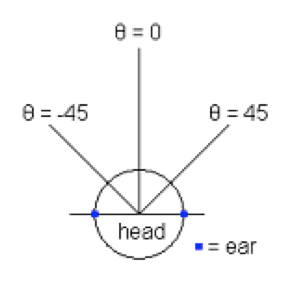
\includegraphics[width=0.4\textwidth]{audio.eps}
\end{center}
\end{figure}

The interaural time between two ears is derived using the formula : Interaural Time Delay (s) = (radius$_{head}$/speed$_{sound}$) $\times (\theta + sin \theta)$, where $\theta$ is expressed in radians. Negative delay indicates that the left ear first hears the sound. 

Note that when =4 or =-4 the ITD for a sound located in front of the head and behind the head are identical. This case is known as the “cone of confusion,” so named after the cone created when this case is projected into a 3D sound space. In natural environments, this confusion is resolved with cues from the outer ear, acoustic variances in the environment, or movement of the head. Unfortunately, we are unable to emulate any of these error-correcting phenomena and therefore cannot differentiate between sounds in front of or behind the head.

We experimented with a sound spatialization algorithm proposed by Birchfield and Gangishetty (2005), but discovered that it yielded identical results to our original algorithm when calculated for the regions of our ConferenceView. For simplicity, we then reverted to the formula above.

\subsection{Volume Difference}
Volume difference is the difference in volume level perceived by the two ears.  According to the distance law, the sound pressure (volume) emitted by a source is inversely proportional to its distance from the listener.

\begin{figure}[htbp]
\begin{center}
    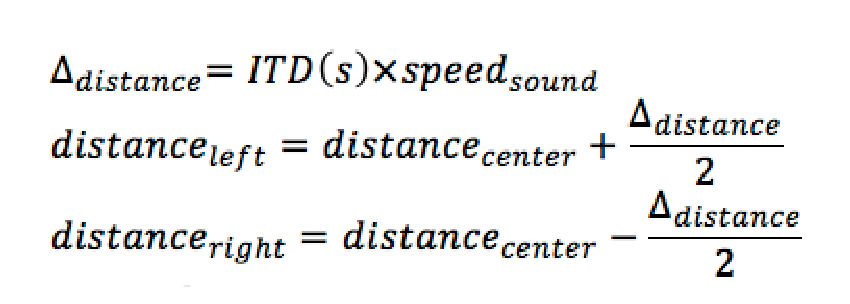
\includegraphics[width=0.4\textwidth]{audio3.eps}
\end{center}
\end{figure}

where distance$_{center}$ is the distance from the sound source to the center of the head. Volume is set for each ear accordingly. Additionally, we simulate the sound shadow caused by the head by muting the muting the opposite ear when the audio source is more than 45 degrees from the center. In the future, we hope to emulate the echo that the muted ear would hear from the environment.

{\footnotesize \bibliographystyle{acm}
\bibliography{paper}}

%Appendix
\clearpage
\onecolumn
\begin{center}
\appendix
\section{Team Members}
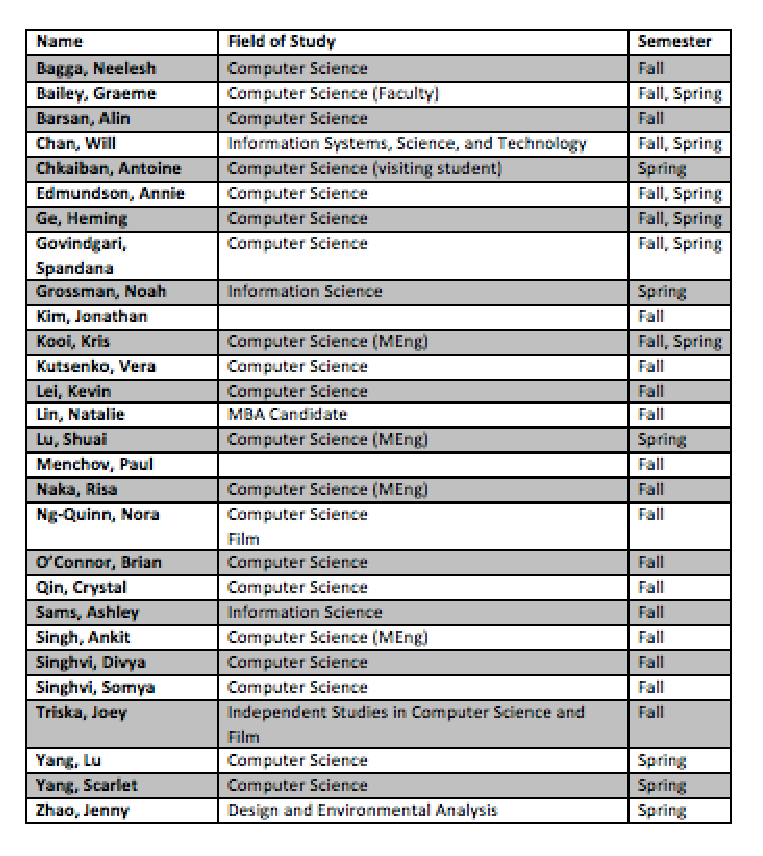
\includegraphics[width=0.6\textwidth]{teammembers.eps}

\clearpage
\section{Design Backlog}
{\raggedright The following are ideas not implemented into the application.  These ideas will not necessarily be in the final application, but they can serve as a starting point for brainstorming.
\begin{itemize}
\item User testing
\item Allowing users to update their personal information and image
\item UI showing users leaving conferences
\item Whisper feature (private conversation with one other member of the conference)
\item Grouping contacts into sublists
\item Enhanced error handling throughout application
\item Security throughout application
\item Integration of audio over the network
\end{itemize}
}
\clearpage
\section{View Management}
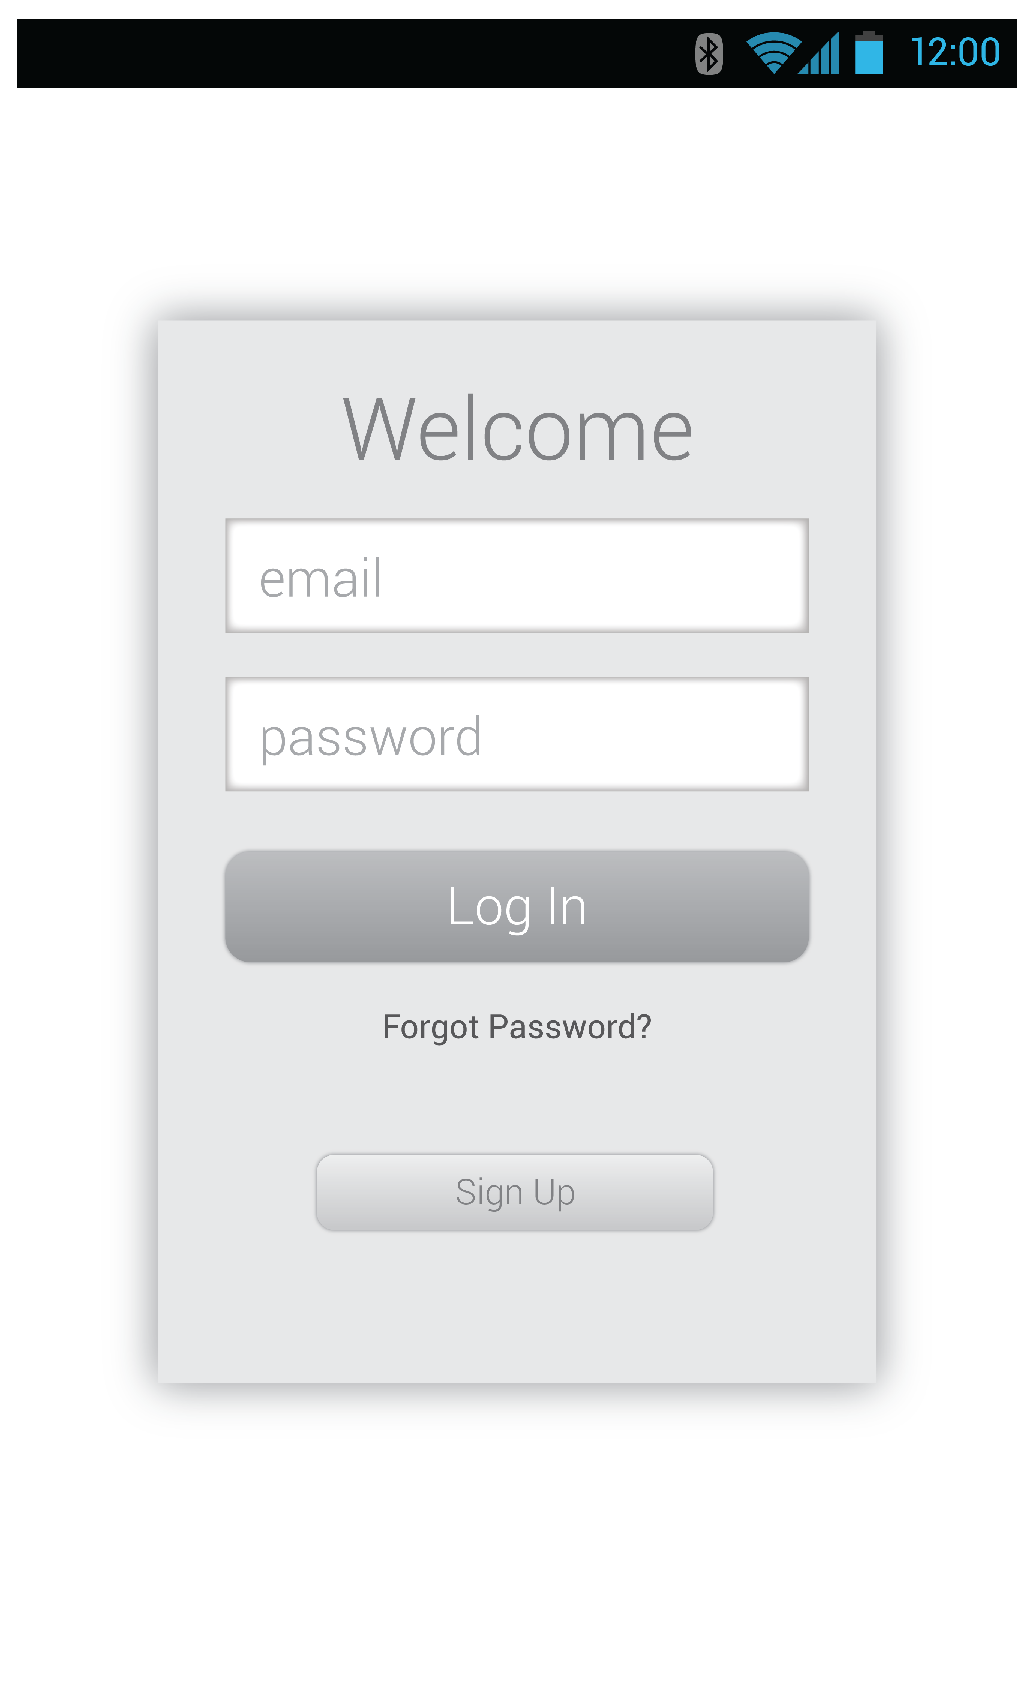
\includegraphics[width=0.6\textwidth]{OpenComm_Login.eps}
\clearpage
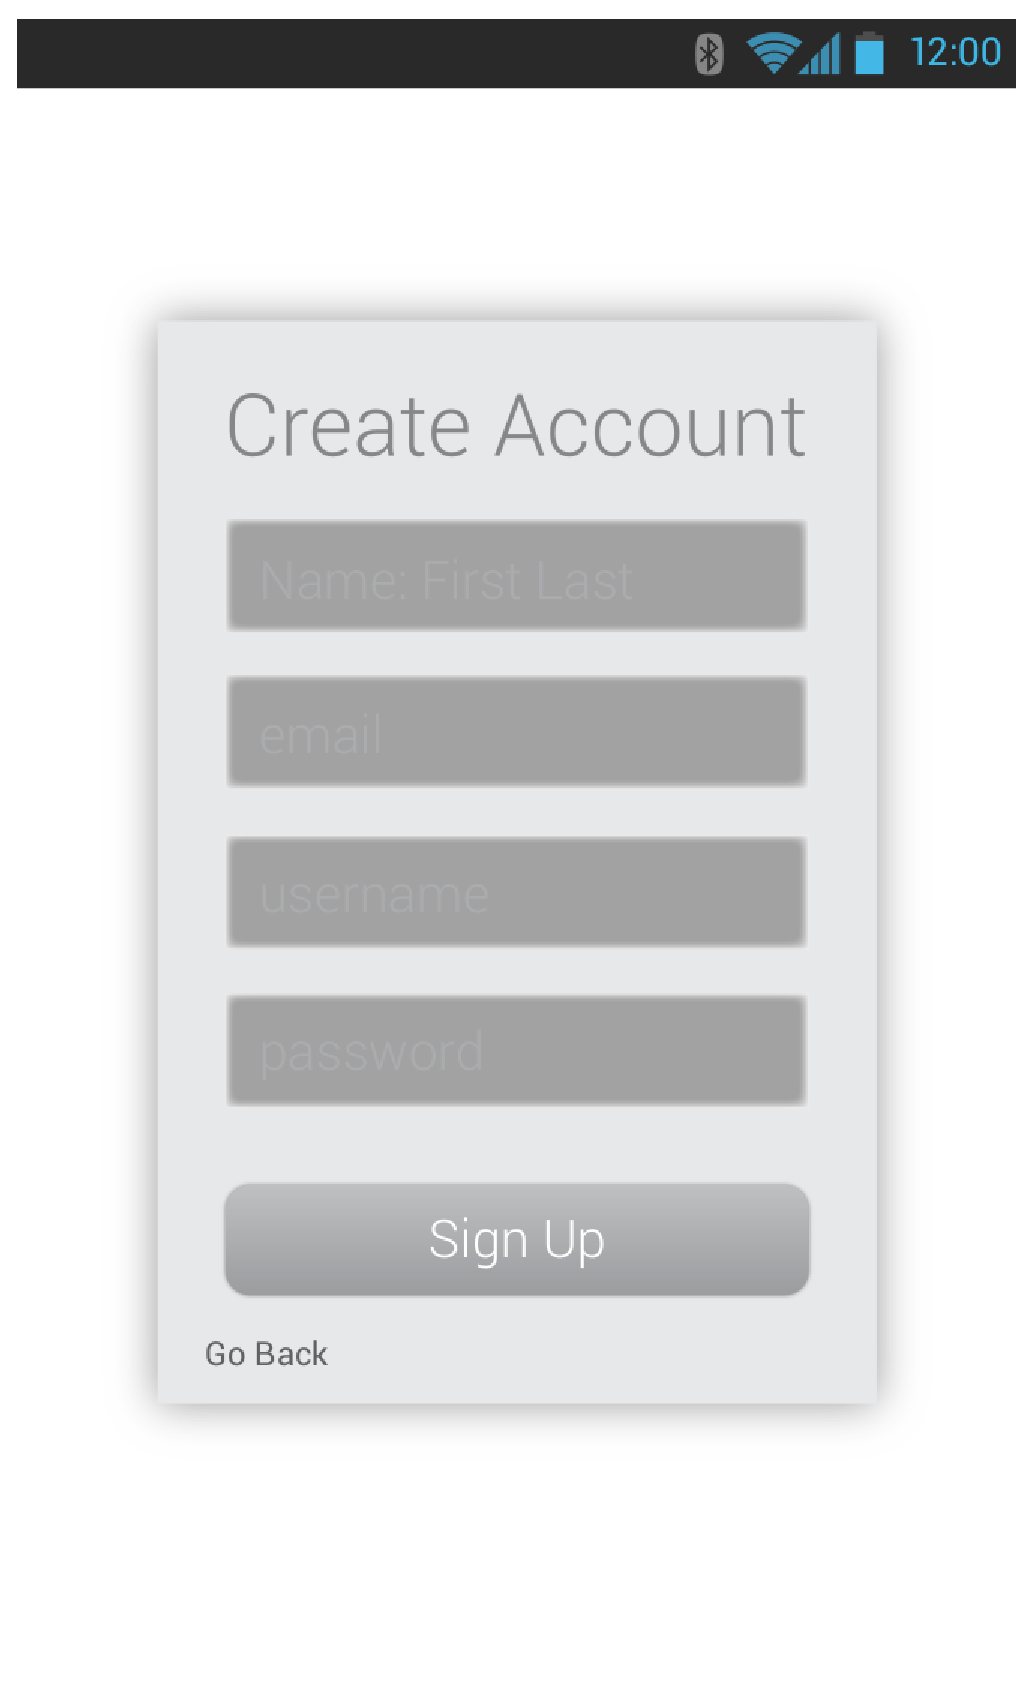
\includegraphics[width=0.6\textwidth]{Create_Account.eps}
\clearpage
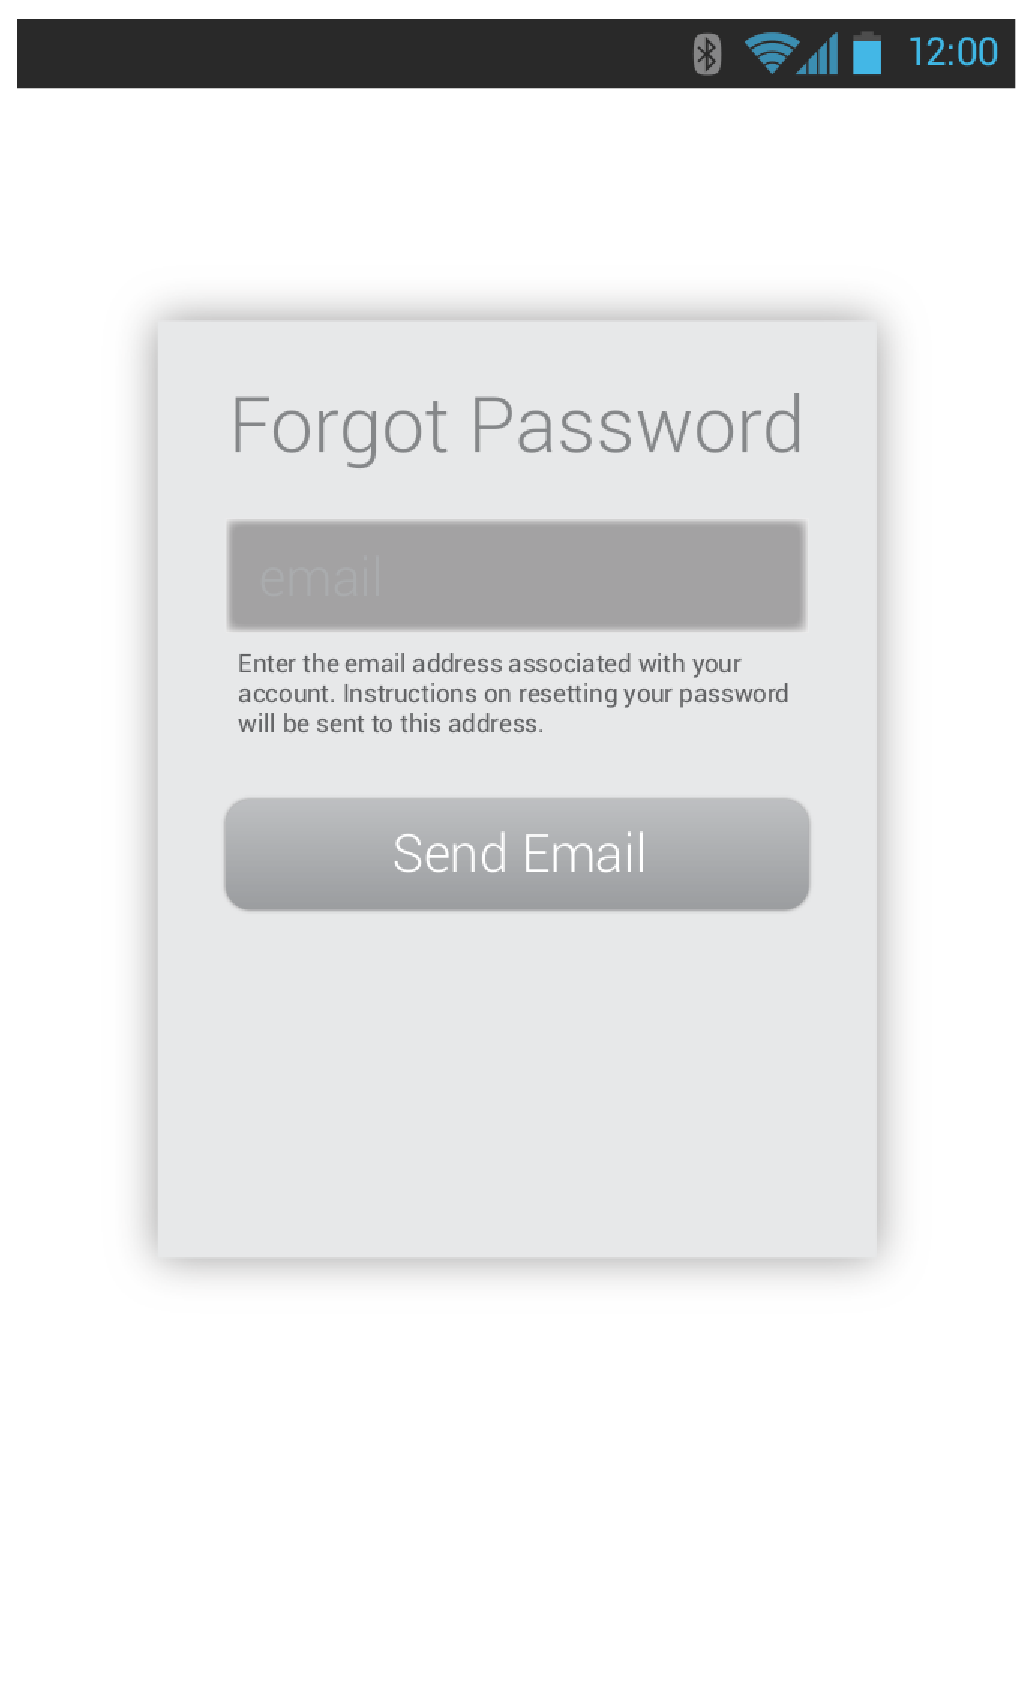
\includegraphics[width=0.6\textwidth]{Forgot_Password.eps}
\clearpage
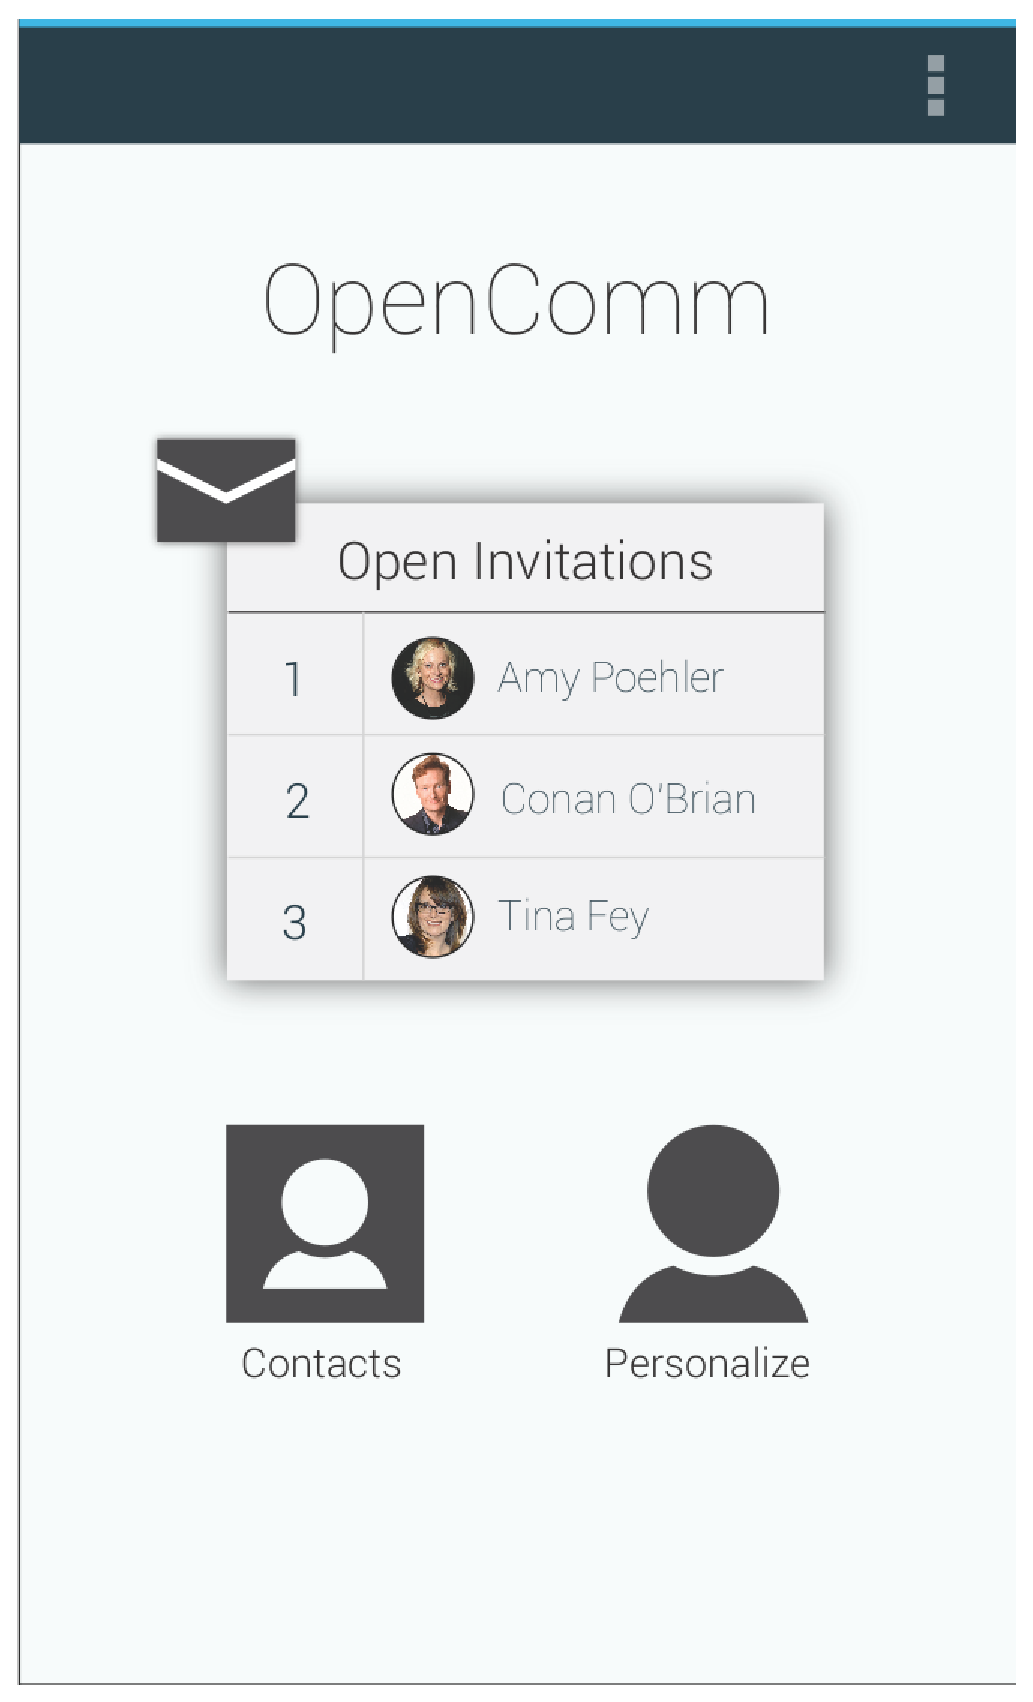
\includegraphics[width=0.6\textwidth]{Dashboard_new.eps}
\clearpage
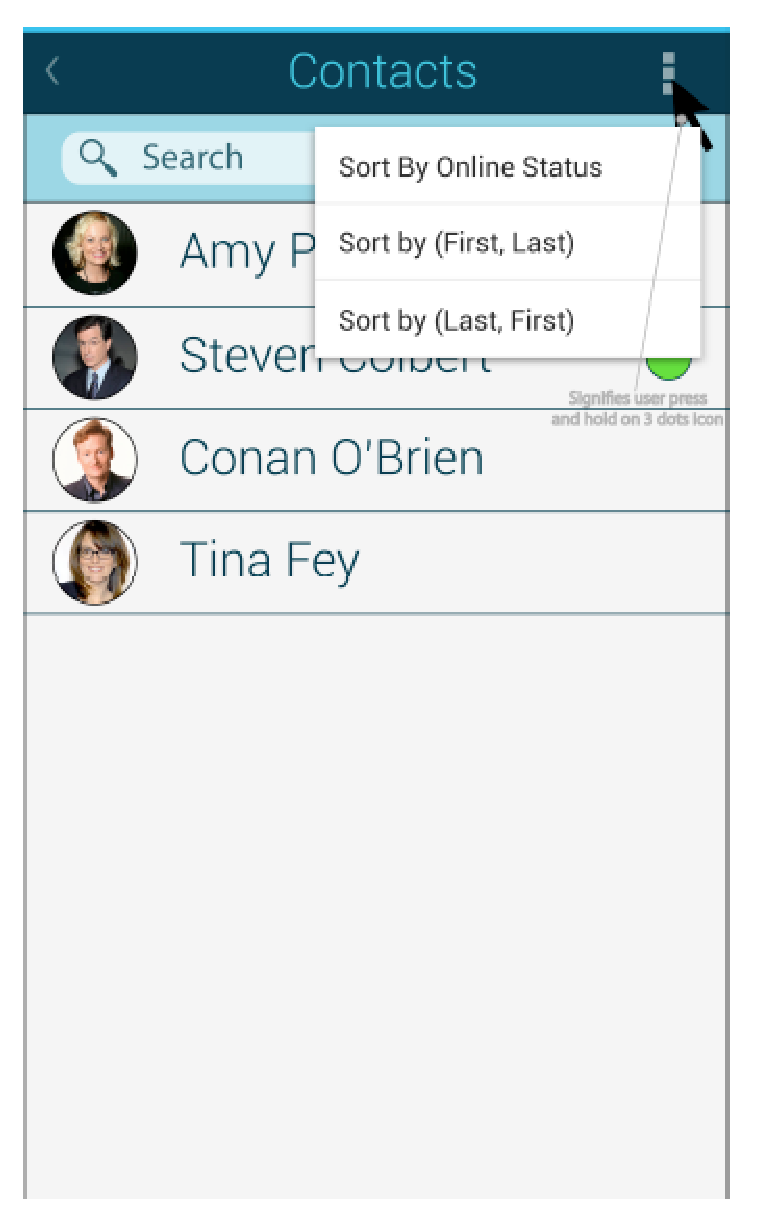
\includegraphics[width=0.6\textwidth]{contacts.eps}
\clearpage
\includegraphics[width=0.6\textwidth]{personalInfo.eps}
\clearpage
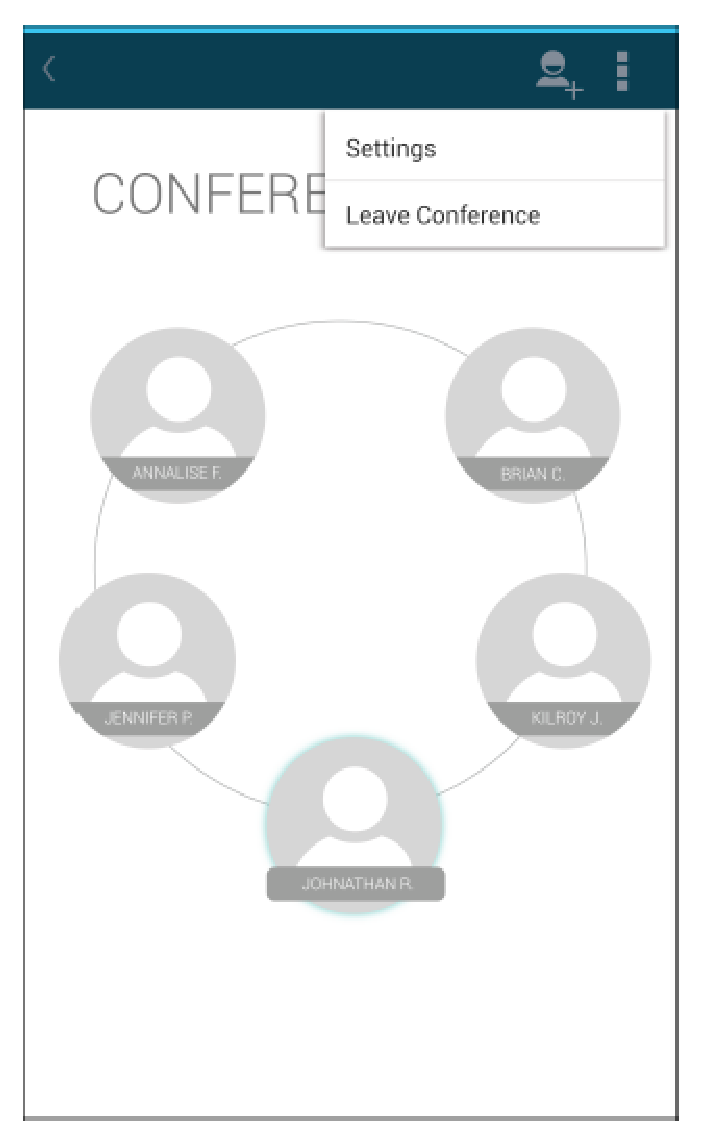
\includegraphics[width=0.6\textwidth]{conference5.eps}

\clearpage
\section{The XMPP Protocol}

\clearpage
\section{Audio, Jingle Protocol, and RTP from Spring 2010 M.Eng. Report}
\end{center}

\end{document}







